
\chapter{Problem statement}
\label{problem}

\section{The NAO Robot}
Aldebaran NAO is a humanoid robot. It is 58 cm tall and it has 5kg approximate mass. The version we are working on is the RoboCup version 3.3 with 21 DOF. It has 2 DOF on the head, 4 on each arm and 5 on each leg and 1 DOF that is common between the two legs. NAO has five kinematic chains and they are the following:
\begin{itemize}
\item Head chain: HeadYaw, HeadPitch.
\item Left Arm chain: LShoulderPitch, LShoulderRoll, LElbowYaw, LElbowRoll.
\item Right Hand chain: RShoulderPitch, RShoulderRoll, RElbowYaw, RElbowRoll.
\item Left Leg chain: LHipYawPitch, LHipRoll, LHipPitch, LKneePitch, LAnklePitch, LAnkleRoll.
\item Right Leg chain: RHipYawPitch, RHipRoll, RHipPitch, RKneePitch, RAnklePitch, RAnkleRoll.
\end{itemize}
The common joint is the HipYawPitch joint, so LHipYawPitch and RHipYawPitch are the same joint.

In the figure bellow we are presenting the academic edition of NAO. NAO RoboCup edition misses 4 DOF on the hand (LWristYaw, LHand, RWristYaw and RHand).
\begin{figure}[h]
	\begin{center}
		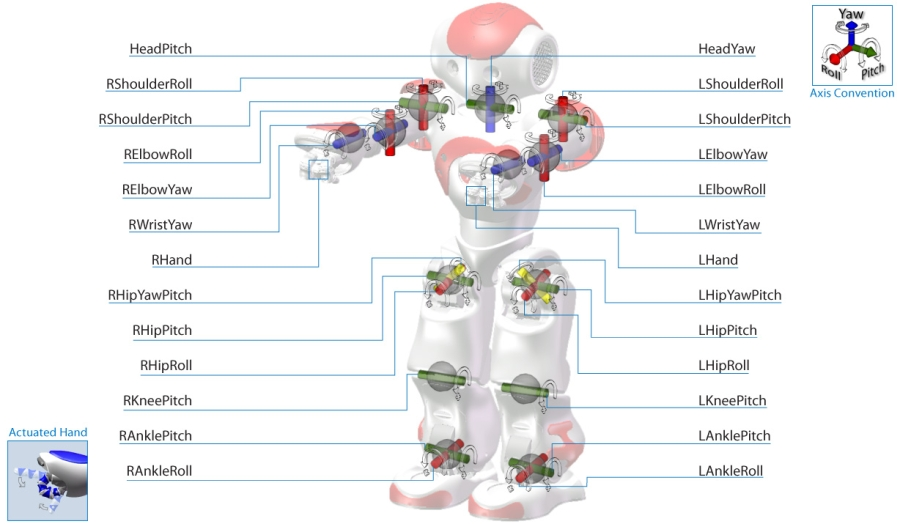
\includegraphics[height = 10cm]{Figures/nao-robot-dof.jpeg}
 		\caption{Aldebaran NAO V3.3 DOF of Academic Edition}
 		\label{fig:NAO}
	\end{center}
\end{figure}
\subsection{NAO Cartesian Restrictions}
In the tables bellow we will present the length of all the links of the robot, the range that each joint is working in radians and in degrees and finally the masses of the NAO. Each joint has its own mass and center of mass. The center of mass for each joint is represented by a point in the three-dimensional space of the joint. The robot theoretically is symmetric but we will see, in the joints ranges, that some left joints have different range than the right ones. The values are extracted from the user manual of the robot that Aldebaran provides.
The user manual has only masses for the right part of the robot but we assume that the robot is fully symmetrical on the masses.
Although some joints appear to be able to go to a position, the hardware controller of the robot will prohibit this movement because of the possible collisions with NAO shell.

\begin{figure}
\begin{tabular}{p{9cm}l|l|}
\multirow{14}{*}{
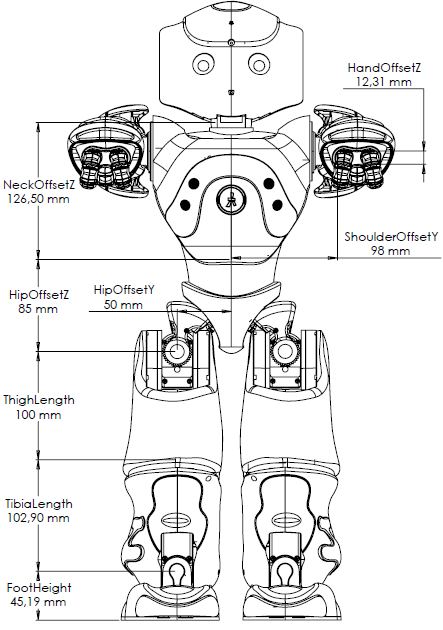
\includegraphics[height = 9cm]{Figures/naolinks_1.png}
}& \multicolumn{2}{c}{} \\
& \multicolumn{2}{c}{} \\
& \multicolumn{2}{c}{} \\
& \multicolumn{2}{c}{} \\
& \multicolumn{2}{c}{} \\
\cline{2-3}
& \multicolumn{1}{|l|}{\textbf{Name}} & \textbf{Size (mm)} \\ \cline{2-3}
& \multicolumn{1}{|l|}{NeckOffsetZ} & 126.50 \\ \cline{2-3}
& \multicolumn{1}{|l|}{ShoulderOffsetY} & 98.00 \\ \cline{2-3}
& \multicolumn{1}{|l|}{ElbowOffsetY} & 15.00 \\ \cline{2-3}
& \multicolumn{1}{|l|}{UpperArmLength} & 105.00 \\ \cline{2-3}
& \multicolumn{1}{|l|}{LowerArmLength} & 55.95 \\ \cline{2-3}
& \multicolumn{1}{|l|}{ShoulderOffsetZ} & 100.00 \\ \cline{2-3}
& \multicolumn{1}{|l|}{HandOffsetX} & 57.75 \\ \cline{2-3}
 & \multicolumn{1}{|l|}{HipOffsetZ} & 85.00 \\ \cline{2-3}
\multirow{10}{*}{
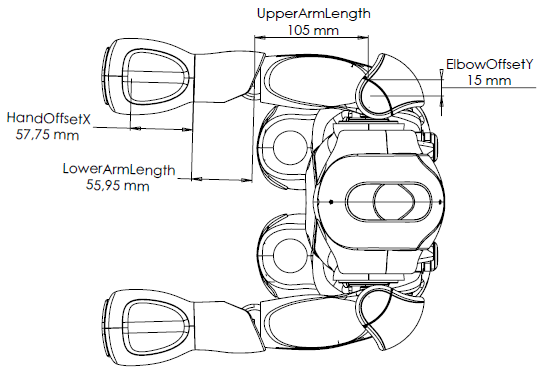
\includegraphics[height = 5cm]{Figures/naolinks_2.png}
}& \multicolumn{1}{|l|}{HipOffsetY} & 50.00 \\ \cline{2-3}
& \multicolumn{1}{|l|}{ThighLength} & 100.00 \\ \cline{2-3}
& \multicolumn{1}{|l|}{TibiaLength} & 102.90 \\ \cline{2-3}
& \multicolumn{1}{|l|}{FootHeight} & 45.19 \\ \cline{2-3}
& \multicolumn{1}{|l|}{HandOffsetZ} & 12.31 \\\cline{2-3}
& \multicolumn{2}{c}{} \\
& \multicolumn{2}{c}{} \\
& \multicolumn{2}{c}{} \\
& \multicolumn{2}{c}{} \\
& \multicolumn{2}{c}{} \\

\end{tabular}
\caption{NAO links sizes}
\label{fig:NAOlinks}
\end{figure}

\begin{figure}
\begin{tabular}{|p{5cm}|p{5cm}|p{5cm}|}
\multicolumn{3}{p{15cm}}{\centering 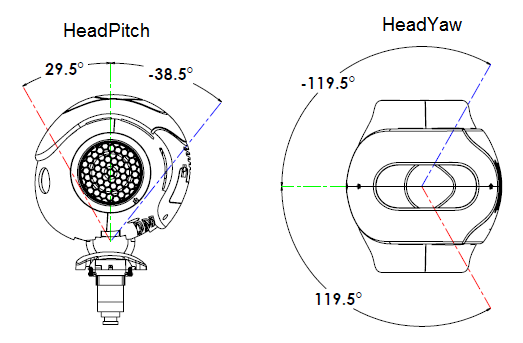
\includegraphics[height = 3.5cm]{Figures/headjoints.png}} \\ \hline
\textbf{Joint Name} & \textbf{Range in Degrees$^{\circ}$} & \textbf{Range in Radians} \\ \hline
HeadYaw & -119.5$^{\circ}$ to 119.5$^{\circ}$ & -2.0857 to 2.0857 \\ \hline
HeadPitch & -38.5$^{\circ}$ to 29.5$^{\circ}$ & -0.6720 to 0.5149 \\ \hline
\end{tabular}
\caption{Head joints range}
\label{fig:hjoints}
\end{figure}

\begin{figure}
\begin{tabular}{|p{5cm}|p{5cm}|p{5cm}|}
\multicolumn{3}{p{15cm}}{\centering 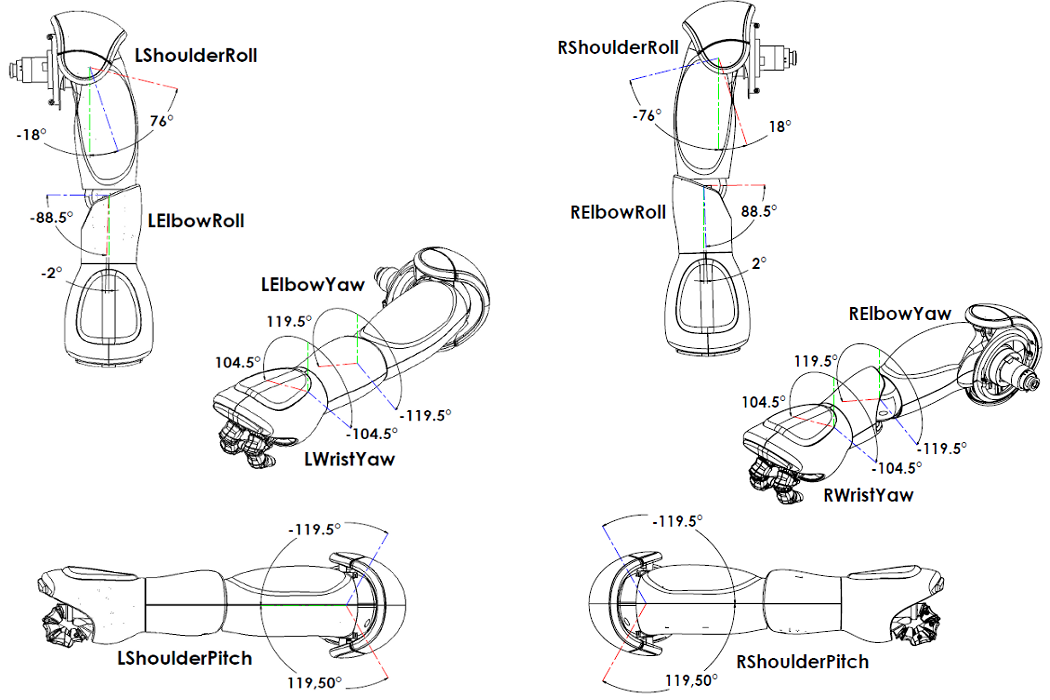
\includegraphics[height = 6.5cm]{Figures/armsjoints.png}} \\ \hline
\textbf{Joint Name} & \textbf{Range in Degrees$^{\circ}$} & \textbf{Range in Radians} \\ \hline
LShoulderPitch & -119.5$^{\circ}$ to 119.5$^{\circ}$ & -2.0857 to 2.0857 \\ \hline
LShoulderRoll & -18$^{\circ}$ to 76$^{\circ}$ & -0.3142 to 1.3265 \\ \hline
LElbowYaw & -119.5$^{\circ}$ to 119.5$^{\circ}$ & 1.5446 to 0.0349 \\ \hline
LElbowRoll & -88.5$^{\circ}$ to -2$^{\circ}$ & -0.6720 to 0.5149 \\ \hline
RShoulderPitch & -119.5$^{\circ}$ to 119.5$^{\circ}$ & -2.0857 to 2.0857 \\ \hline
RShoulderRoll & -38.5$^{\circ}$ to 29.5$^{\circ}$ & -1.3265 to 0.3142 \\ \hline
RElbowYaw & -119.5$^{\circ}$ to 119.5$^{\circ}$ & -2.0857 to 2.0857 \\ \hline
RElbowRoll & -38.5$^{\circ}$ to 29.5$^{\circ}$ & 0.0349 to 1.5446 \\ \hline
LWristYaw and RWristYaw & disabled & disabled \\ \hline
\end{tabular}
\caption{Arms joints range}
\label{fig:ajoints}
\end{figure}

\begin{figure}
\begin{tabular}{|p{5cm}|p{5cm}|p{5cm}|}
\multicolumn{3}{p{15cm}}{\centering 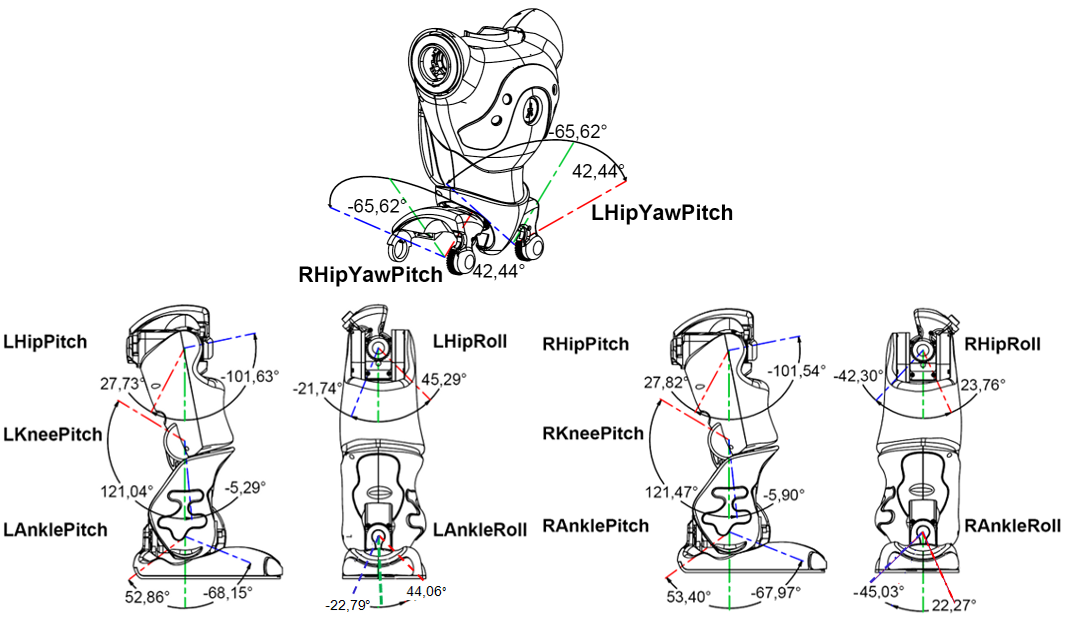
\includegraphics[width = 15cm]{Figures/legsjoints.png}} \\ \hline
\textbf{Joint Name} & \textbf{Range in Degrees$^{\circ}$} & \textbf{Range in Radians} \\ \hline
LHipYawPitch-RHipYawPitch & -65.62 to 42.44 & -1.145303 to 0.740810 \\ \hline
LHipRoll & -21.74$^{\circ}$ to 45.29$^{\circ}$ & -0.379472 to 0.790477 \\ \hline
LHipPitch & -101.63$^{\circ}$ to 27.73$^{\circ}$ & -1.773912 to 0.484090 \\ \hline
LKneePitch & -5.29$^{\circ}$ to 121.04$^{\circ}$ & -0.092346 to 2.112528 \\ \hline
LAnklePitch & -68.15$^{\circ}$ to 52.86$^{\circ}$ & -1.189516 to 0.922747 \\ \hline
LAnkleRoll & -22.79$^{\circ}$ to 44.06$^{\circ}$ & -0.397880 to 0.769001 \\ \hline
RHipRoll & -42.30$^{\circ}$ to 23.76$^{\circ}$ & -0.738321 to 0.414754 \\ \hline
RHipPitch & -101.54$^{\circ}$ to 27.82$^{\circ}$ & -1.772308 to 0.485624 \\ \hline
RKneePitch & -5.90$^{\circ}$ to 121.47$^{\circ}$ & -0.103083 to 2.120198 \\ \hline
RAnklePitch & -67.97$^{\circ}$ to 53.40$^{\circ}$ & -1.186448 to 0.932056 \\ \hline
RAnkleRoll & -45.03$^{\circ}$ to 22.27$^{\circ}$ & -0.785875 to 0.388676 \\ \hline
\end{tabular}
\caption{Legs joints range}
\label{fig:ljoints}
\end{figure}

\begin{table}[position specifier]
\caption{Masses of NAO}
\begin{tabular}{|l|r|r|r|r|}
\hline
\multicolumn{5}{|c|}{\textbf{Masses for NAO v3.3 robocup edition (H21)}} \\ \hline
\multicolumn{3}{|l|}{Total Mass For NAO H21} & \multicolumn{2}{|r|}{4.879 kg}\\ \hline
\textbf{Frame Name} & \textbf{Mass (Kg)} & \textbf{CoM$_{\text{x}}$ (mm)} & \textbf{CoM$_{\text{y}}$ (mm)} & \textbf{CoM$_{\text{z}}$ (mm)}\\ \hline
Torso & 1.03948 & -4.15 & 0.07 & 42.58 \\ \hline
HeadYaw & 0.05930 & -0.02 & 0.17 & 25.56 \\ \hline
HeadPitch & 0.52065 & 1.2 & -0.84 & 53.53 \\ \hline
RShoulderPitch & 0.06996 & -1.78 & 24.96 & 0.18 \\ \hline
RShoulderRoll & 0.12309 & 18.85 & -5.77 & 0.65 \\ \hline
RElbowYaw & 0.05971 & -25.6 & 0.01 & -0.19 \\ \hline
RElbowRoll & 0.185 & 65.36 & -0.34 & -0.02 \\ \hline
LShoulderPitch & 0.06996 & -1.78 & -24.96 & 0.18 \\ \hline
LShoulderRoll & 0.12309 & 18.85 & 5.77 & 0.65 \\ \hline
LElbowYaw & 0.05971 & -25.6 & -0.01 & -0.19 \\ \hline
LElbowRoll & 0.185 & 65.36 & 0.34 & -0.02 \\ \hline
RHipYawPitch & 0.07117 & -7.66 & 12 & 27.17 \\ \hline
RHipRoll & 0.1353 & -16.49 & -0.29 & -4.75 \\ \hline
RHipPitch & 0.39421 & 1.32 & -2.35 & -53.52 \\ \hline
RKneePitch & 0.29159 & 4.22 & -2.52 & -48.68 \\ \hline
RAnklePitch & 0.13892 & 1.42 & -0.28 & 6.38 \\ \hline
RAnkleRoll & 0.16175 & 25.4 & -3.32 & -32.41 \\ \hline
LHipYawPitch & 0.07117 & -7.66 & -12 & 27.17 \\ \hline
LHipRoll & 0.1353 & -16.49 & 0.29 & -4.75 \\ \hline
LHipPitch & 0.39421 & 1.32 & 2.35 & -53.52 \\ \hline
LKneePitch & 0.29159 & 4.22 & 2.52 & -48.68 \\ \hline
LAnklePitch & 0.13892 & 1.42 & 0.28 & 6.38 \\ \hline
LAnkleRoll & 0.16175 & 25.4 & 3.32 & -32.41 \\ \hline
\end{tabular}
\label{tab:Masses of NAO}
\end{table}

\newpage
\section{Kinematics for NAO}
Because NAO has a lot of DOF, it can do several complex moves. Some examples of those complex moves are walking, kicking a ball, standing up etc. NAO has five kinematic chains, three of them completely independent and two of them with one common joint. Kinematics is very useful for the programmers of NAO because they can create dynamic movements with the use of inverse kinematics or they can find the horizon of the camera on the head of the robot using forward kinematics.
\subsection{The Forward Kinematics problem for NAO}
Forward kinematics for NAO can been seen as five individual solutions. NAO has five chains and because we will not manipulate the joints, but we will only take the current state of each joint, we can assume that the five chains are completely independent. Then, we can find five forward kinematics solutions, one for each kinematic chain and we will be able to combine these solutions to find a solution for a bigger kinematic chain (e.g. the kinematic chain from the right foot to the head). The reason for dealing with this problem is twofold:firstly it is of great importance (concerning many applications, such as, finding its horizon, as well as placing it correctly).Besides this, as it will be described below, solution to the inverse kinematics problem would be intractable without solving the forward first.

\subsection{The Inverse Kinematics problem for NAO}
The inverse kinematics problem is a more complex problem and although we have the common joint between two kinematic chains, we are working with the assumption that we have five completely independent kinematic chains, so we will find five solutions for this problem. The reasons that led us to solve it are many. More specifically, we need to create dynamic kicks and an omni-directional walk. Both problems need a mechanism to move trajectories from the \(three-dimensional\) space to the \(joint\) space and the inverse kinematics can provide this mechanism.
\subsubsection*{Analytic versus Approximate solutions}
Inverse kinematics problem can be solved analytically or approximately. We have chosen to find the analytical solution rather than the approximate solution because the second one has some problems. We need real-time execution to the problem of inverse kinematics. The analytical solution is faster than the fastest approximate solution and for this reason it is a good choice for real-time execution. Second, there are various implementations of approximate solutions for the problem. Some of them are fast but it is very possible to run into a singularity. Other methods have a smaller probability to run into a singularity, but they are slower. On the other hand, the analytical solution doesn't have any singularity. However, inverse kinematics have an analytical solution only if the chain has five or less DOF. If the chain has 6 DOF, it can have analytical solution to the problem of the inverse kinematics only if three sequential joints have intersecting axes.
% ------------------------------------------------------------------------

%%% Local Variables:
%%% mode: latex
%%% TeX-master: "../thesis"
%%% End:
